%%%%%%%%%%%%%%%%%%%%%%%%%%%%%%%%%%%%%%%%%%%%%%%%%%%%%%%%%%%%%%%%%%%%%%%%%%%%%
%
%  System        : 
%  Module        : 
%  Object Name   : $RCSfile$
%  Revision      : $Revision$
%  Date          : $Date$
%  Author        : $Author$
%  Created By    : Robert Heller
%  Created       : Sat Apr 15 10:37:45 2023
%  Last Modified : <230415.1645>
%
%  Description 
%
%  Notes
%
%  History
% 
%%%%%%%%%%%%%%%%%%%%%%%%%%%%%%%%%%%%%%%%%%%%%%%%%%%%%%%%%%%%%%%%%%%%%%%%%%%%%
%
%    Copyright (C) 2023  Robert Heller D/B/A Deepwoods Software
%			51 Locke Hill Road
%			Wendell, MA 01379-9728
%
%    This program is free software; you can redistribute it and/or modify
%    it under the terms of the GNU General Public License as published by
%    the Free Software Foundation; either version 2 of the License, or
%    (at your option) any later version.
%
%    This program is distributed in the hope that it will be useful,
%    but WITHOUT ANY WARRANTY; without even the implied warranty of
%    MERCHANTABILITY or FITNESS FOR A PARTICULAR PURPOSE.  See the
%    GNU General Public License for more details.
%
%    You should have received a copy of the GNU General Public License
%    along with this program; if not, write to the Free Software
%    Foundation, Inc., 675 Mass Ave, Cambridge, MA 02139, USA.
%
% 
%
%%%%%%%%%%%%%%%%%%%%%%%%%%%%%%%%%%%%%%%%%%%%%%%%%%%%%%%%%%%%%%%%%%%%%%%%%%%%%

\subsection{Yard Throat with track selector}
\label{sect-appl:yardthroat}

\begin{figure}[hbpt]\begin{centering}%
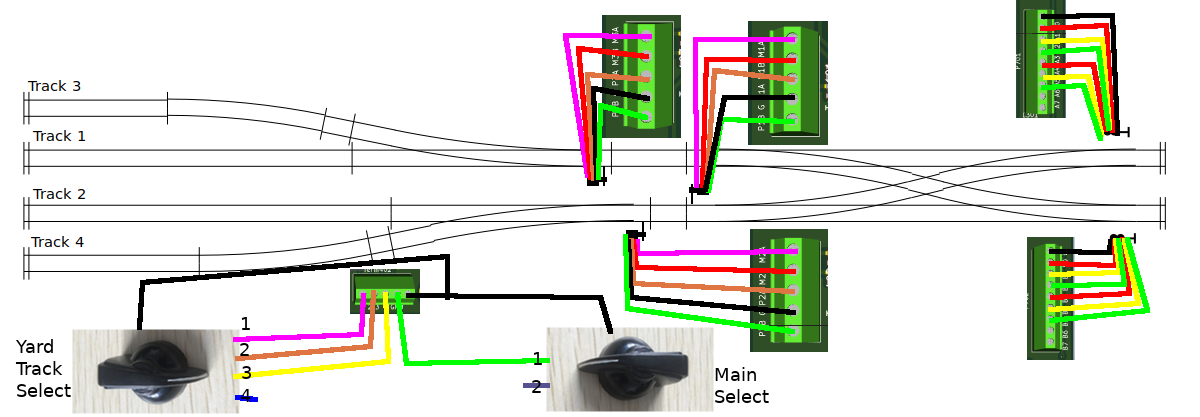
\includegraphics[width=5in]{YardThroat_TrackSelector.png}
\caption{Yard throat with yard ladders and selectors.}
\label{fig:YardThroatTrackSelector}
\end{centering}\end{figure}

This is the entrance to a yard from a double track main line with a sissors 
type crossover and a simple yard ladder.  There are two selector switches, one 
to select the main track and one to select the yard track.  There are a pair 
of signals at the yard entrance, one for each main line track.  These are 3 
over 3 signals.  The basic wiring is shown in 
Figure~\ref{fig:YardThroatTrackSelector}. We will use three turnout drivers 
(the Stall Motor daughter board is shown, but any of the daughter 
boards could be used), 12 of the signal lamp driver outputs, and all four of 
the button inputs.

We will start by configuring the user name and description of the node in User 
Info tab.  When we have done this will will be able to find the node by 
looking for the name.  

Next, we will move onto the Board Configuration tab and give names to the 
Turnout and Points we will be using.

Then we will move onto the button inputs.  The rotary switches total 6 
positions, but we can get by with only 4 inputs, by leaving one position of 
each switch unconnected.  This works because we get extra state information in 
the form of ``none of the above'' -- when all three of buttons 1, 2, and 3 are 
``off'', yard track 4 is selected and when button 4 is off, main track 2 is 
selected.

The logic for the yard track selection is:

\begin{verbatim}
if button1 is on then
  track 1 selected
else if button2 is on then
  track 2 selected
else if button3 is on then
  track 3 selected
else
  track 4 selected
\end{verbatim}

and the logic for the main track selection is:

\begin{verbatim}
if button4 is on then
  main track 1 selected
else
  main track 2 selected
\end{verbatim}

The logic for the sissors crossover is:

\begin{verbatim}
if ( track 1 selected OR track 3 selected) AND 
   main track 1 selected then
  NORMAL
else if ( track 1 selected OR track 3 selected) AND 
        main track 2 selected then
  REVERSE
else if ( track 2 selected OR track 4 selected) AND 
        main track 1 selected then
  REVERSE
else if ( track 2 selected OR track 4 selected) AND 
        main track 2 selected then
  NORMAL
\end{verbatim}

This \textit{look} formidable, but we can simplify things using a ``trick'' --
a kind of ``wired or'', by using a common event id to represent a common 
routing for the odd and even yard tracks.  This simplifies things to

\begin{verbatim}
if common odd tracks AND main track 1 selected then
  NORMAL
else if common odd tracks AND main track 2 selected then
  REVERSE
else if common even tracks AND main track 1 selected then
  REVERSE
else if common even tracks AND main track 2 selected then
  NORMAL
\end{verbatim}


